\documentclass[11pt,a4paper]{article}
\usepackage[utf8]{inputenc}
\usepackage[T1]{fontenc}
\usepackage{lmodern}
\usepackage[margin=2.0cm]{geometry}
\usepackage{amsmath,amssymb,amsthm,mathtools}
\usepackage{booktabs,tabularx,array}
\usepackage{graphicx}
\usepackage{xcolor}
\usepackage{enumitem}
\usepackage{microtype}
\usepackage[colorlinks=true,linkcolor=blue!55!black,citecolor=blue!55!black,urlcolor=blue!55!black]{hyperref}

\renewcommand{\abstractname}{Kivonat}
\renewcommand{\contentsname}{Tartalomjegyzék}
\renewcommand{\figurename}{Ábra}
\renewcommand{\tablename}{Táblázat}
\renewcommand{\refname}{Irodalomjegyzék}
\renewcommand{\proofname}{Bizonyítás}

\setlength{\emergencystretch}{3em}
\newtheorem{theorem}{Tétel}[section]
\newtheorem{proposition}[theorem]{Állítás}
\newtheorem{remark}[theorem]{Megjegyzés}

\title{\textbf{Töltött fermionok tömeghierarchiája, Koide-ekvipartíció\\
és zérus szabad paraméteres \texorpdfstring{$\mathrm{CKM}$}{CKM}-zárás egy tetraéderes\\
\texorpdfstring{$\mathrm{Spin}(10) \to \mathrm{Pati\text{--}Salam} \to \mathrm{SM}$}{Spin(10) -> Pati-Salam -> SM} renormalizációs toronyból}\\[0.35em]
\large Kéthurkos mátrix-\texorpdfstring{$\mathrm{RGE}$}{RGE}-k, mértékinvariáns \texorpdfstring{$G_{\mathrm{PS}}$}{GPS} \texorpdfstring{$y_b/y_\tau$}{yb/ytau}-stabilizáció és egzakt No-Go tételek (\texttt{Paper 25}, \texttt{v1.1.0})}

\author{\textbf{Olcsák József}\\
\small Független kutató $\cdot$ ORCID: \href{https://orcid.org/0009-0003-7311-6522}{0009-0003-7311-6522}\\
\small E-mail: \href{mailto:jolcsak@gmail.com}{jolcsak@gmail.com}}
\date{2026.\ november 20.}

\begin{document}
\maketitle

\begin{abstract}
\noindent A Standard Modell (SM) töltött fermion-szektorának tizenhárom íz-paraméterét --- kilenc töltött lepton- és kvarktömeget, valamint négy Cabibbo--Kobayashi--Maskawa (CKM) keveredési paramétert --- nem-szuperszimmetrikus nagy egyesítési (GUT) modellekben szigorú renormalizációs-csoport (RG) és csoportelméleti akadályok terhelik: a minimális $y_b = y_\tau$ egyesülés kudarca, a Koide-reláció sugárzási érzékenysége, valamint a $\mathrm{Spin}(10)$ Yukawa-szektor szinguláris-érték korlátai. Tanulmányunkban teljes kéthurkos SM és mértékinvariáns Pati--Salam RG- és ábrázoláselméleti auditot végzünk a négycsúcsú tetraéderes ($K_4$, $N = 4$) operátor-invariánsok ($(d_S, d_A, d_{\mathrm{full}}) = (3, 8, 9)$, $\lambda_q \equiv 2/d_{\mathrm{full}} = 2/9$, $\sin^2\theta_W^{\mathrm{UV}} = d_S/d_A = 3/8$) és az $M_{\mathrm{PS}} = 3.66\times 10^{11}\;\mathrm{GeV}$, $M_R = 5.565\times 10^{14}\;\mathrm{GeV}$ köztes küszöbskálák mentén. (1) Szimbolikus algebrával (\texttt{SymPy}) igazoljuk, hogy bármely Hermitikus cirkuláns $S_\ell \in \mathrm{End}(V_3)$ flavonra ($Y_e \propto S_\ell^2$) a Koide-féle $Q = 2/3$ feltétel ekvivalens az egzakt Frobenius-norma ekvipartícióval ($\|\tilde{S}_\ell\|_F^2 = \|S_{\ell,0}\|_F^2$, $r = 1/\sqrt{2}$), és egy nyomcsere-szimmetrikus kvartikus potenciál szigorú globális minimuma; a $\theta = 2/d_{\mathrm{full}} = 2/9\;\mathrm{rad}$ fázissal $m_\mu/m_e = 206.7703$ ($+0.0010\%$) és $m_\tau/m_\mu = 16.8180$ ($+0.0060\%$), míg a teljes kéthurkos SM RG-futás $M_Z \to M_*$ között mindössze $+3.66\times 10^{-6}$-tal tolja el $Q_e$-t. (2) Három egzakt No-Go tételt bizonyítunk: a tiszta kéthurkos SM-sivatagban a $-108\,g_3^4$ QCD-tag $y_b(M_R)/y_\tau(M_R) = 0.6173$-ra nyomja le az arányt ($+9.12\sigma_{\mathrm{exp}}$ feszültség $2/3$-hoz képest); a valódi valós $\mathbf{10}_H \oplus \overline{\mathbf{126}}_H$ ($|v_u^{(10)}/v_d^{(10)}| = 1$) még hatfázisú Autonne--Takagi átfázisolás mellett is globálisan kizárt; a szimmetrikus $(1,3)=0$ Fritzsch-textúrák pedig $1.98\times$-osan alábecsülik a $|V_{ub}|/|V_{cb}|$ arányt. (3) A $D$-paritás-sértett $\mathrm{Spin}(10) \xrightarrow{M_{\mathrm{GUT}}} G_{\mathrm{PS}}\times D \xrightarrow{M_R} G_{\mathrm{PS}} \xrightarrow{M_{\mathrm{PS}}} G_{\mathrm{SM}}$ láncban --- a Schur-lemma által megkövetelt $\Phi_{15}(\mathbf{15},\mathbf{2},\mathbf{2})$ megtartásával ($b_{\mathrm{PS}} = (-5/3, +2, +26/3)$) --- a manifeszt $G_{\mathrm{PS}}$-invariáns bidublett Yukawa RGE-k kioltják mind a mérték-, mind az $\mathcal{O}(y_t^2)$ fermionláb-hasadást $Y_1$ és $Y_{15}$ között, $y_b(M_R)/y_\tau(M_R) = 0.6937$-re rögzítve az arányt ($+4.06\%$ a $2/3$-tól). Szimmetrikus komplex $\mathbf{10}_H \oplus \overline{\mathbf{126}}_H$ mátrixokkal --- csupán a két 3.\ generációs skálát $(y_t, y_\tau)$ rögzítve, $0$ szabad íz-paraméterrel --- mind a tíz független kvarktömeg és CKM-megfigyelhető $\le 2.85\sigma_{\mathrm{tot}}$ határon belülre esik $M_Z$-nél ($p_{\mathrm{LEE}} = 9.98\times 10^{-5}$ a keveretlen $G_{\mathrm{PS}}$ tornyon és $1.92\times 10^{-6}$ a kéthurkos sivatagban).
\end{abstract}

\tableofcontents
\vspace{0.4em}
\hrule
\vspace{0.8em}

\section{Bevezetés és episztemikus határok}

A Standard Modell tizenhárom töltött-fermion íz-paraméterének nem-szuperszimmetrikus egyesítése négy elméleti akadályba ütközik \cite{PDG2024,Cabibbo1963,KobayashiMaskawa1973,PatiSalam1974,FritzschMinkowski1975,GeorgiJarlskog1979,MaRajasekaran2001,AltarelliFeruglio2010}: (1) a Koide-reláció ($Q_{\mathrm{pole}} = 0.6666605 \simeq 2/3$, $\theta \simeq 2/9$) \cite{Koide1983,Brannen2006} alacsony energiájú QED-eltolódása $\overline{\mathrm{MS}}$-ben \cite{Sumino2009,XingZhangZhou2012}; (2) a kéthurkos QCD $-108\,g_3^4$ futás által okozott $y_b/y_\tau$ zuhanás a tiszta SM-sivatagban \cite{Arason1992,HuangZhou2021,AntuschSpinrath2009,AntuschMaurer2013}; (3) a valódi valós $\mathbf{10}_H \oplus \overline{\mathbf{126}}_H$ $\mathrm{Spin}(10)$ modell ($|v_u^{(10)}|=|v_d^{(10)}|$) \cite{BabuMohapatra1993,BajcSenjanovicVissani2006,DueckRodejohann2013} és a $(1,3)=0$ Fritzsch-textúrák \cite{Fritzsch1978,RobertsRomaninoRoss2001} kudarca; valamint (4) a Look-Elsewhere túlillesztés veszélye.

A négycsúcsú tetraéderes ($K_4$, $N = 4$) szimpliciális-Clifford keretrendszerben \cite{Olcsak2026Zenodo,Olcsak2026Paper24} a $V_3$ standard ábrázolás dimenziói $(d_S, d_A, d_{\mathrm{full}}) = (3, 8, 9)$ rögzítik a $\lambda_q = 2/d_{\mathrm{full}} = 2/9$ és $\sin^2\theta_W^{\mathrm{UV}} = d_S/d_A = 3/8$ arányokat, valamint a skálatornyot:
\begin{equation}
M_* = \frac{M_{\mathrm{Pl}}}{\sqrt{3}} = 1.4060\times 10^{18}\;\mathrm{GeV}, \qquad
M_R = \frac{M_*}{256\pi^2} = 5.5649\times 10^{14}\;\mathrm{GeV}, \qquad
M_{\mathrm{PS}} = 3.66\times 10^{11}\;\mathrm{GeV}.
\end{equation}
Munkánkban szigorúan elkülönítjük a feltétel nélküli matematikai/QFT tételeket és No-Go pajzsokat az explicit diszkrét UV-peremfeltételektől (\texttt{BC-UV-FLAV-1/2/3}) és a két rögzítetlen 3.\ generációs skálától ($y_t(M_R)$, $y_\tau(M_R)$).

\section{Töltött leptonok: Frobenius-ekvipartíció és RG-stabilitás}

\begin{theorem}[Frobenius-ekvipartíció és egzakt Hesse-minimum]
Legyen $S_\ell = S_{\ell,0} + \tilde{S}_\ell \in \mathrm{End}(V_3)$ Hermitikus cirkuláns flavon ($S_{\ell,0} = c_0 I_3$, $\mathrm{Tr}\,\tilde{S}_\ell = 0$, mellékátlós amplitúdó $r e^{\pm i\theta}$) és $Y_e = \Lambda_\ell^{-2} S_\ell^2$ \cite{Koide1990,Sumino2009}. Ekkor $s_k \ge 0$ esetén:
\begin{equation}
Q(Y_e) = \frac{\mathrm{Tr}(S_\ell^2)}{(\mathrm{Tr}\,S_\ell)^2} = \frac{1 + 2r^2}{3} = \frac{2}{3}
\quad\Longleftrightarrow\quad r = \frac{1}{\sqrt{2}}
\quad\Longleftrightarrow\quad \|\tilde{S}_\ell\|_F^2 = \|S_{\ell,0}\|_F^2.
\end{equation}
A $V(S_\ell) = -\mu^2\mathrm{Tr}(S_\ell^2) + \lambda_1[\mathrm{Tr}(S_\ell^2)]^2 + \lambda_2[\mathrm{Tr}(\tilde{S}_\ell^2) - \frac{1}{3}(\mathrm{Tr}\,S_\ell)^2]^2$ ($\lambda_1,\lambda_2 > 0$) potenciál szigorú globális minimuma az $r = 1/\sqrt{2}$, $c_0 = \sqrt{\mu^2/(12\lambda_1)}$ Koide-sokaság, egzakt Hesse-elemekkel:
\begin{equation}
H_{c_0 c_0} = 24\mu^2, \qquad
H_{rr} = \frac{(\lambda_1 + \lambda_2)\mu^4}{\lambda_1^2}, \qquad
H_{c_0 r} = \frac{2\sqrt{6}\,\mu^3}{\sqrt{\lambda_1}}, \qquad
\det H_{(c_0,r)} = \frac{24\lambda_2 \mu^6}{\lambda_1^2} > 0.
\end{equation}
\end{theorem}

\begin{remark}[UV szimmetriafeltételek]
A potenciál az $\Lambda_\ell \gtrsim M_{\mathrm{PS}}$ UV-skálán (i) nyom--nyommentes csere-szimmetriát ($\mu_0^2 = \tilde{\mu}^2$, $\lambda_{00} = \lambda_{\tilde{}\tilde{}}$) és (ii) az $\mathrm{U}(1)_\theta$ explicit sérülését feltételezi (elkerülve a tömegtelen Goldstone-familont), a $(\mathrm{Tr}\,S_\ell)\mathrm{Tr}(\tilde{S}_\ell^3) \propto \cos 3\theta$ köbös operátor elnyomásával. A diszkrét $\theta = \lambda_q = 2/9\;\mathrm{rad}$ (\texttt{BC-UV-FLAV-1}) peremfeltétellel $m_\mu/m_e = 206.7703$ ($+0.0010\%$), $m_\tau/m_\mu = 16.8180$ ($+0.0060\%$) és $m_\tau/m_e = 3477.47$ ($+0.0070\%$) (\ref{fig:koide_hu}.~ábra).
\end{remark}

\begin{theorem}[16 nagyságrendű SM RG-stabilitás és Sumino-féle IR-QED pajzs]
Teljes kéthurkos SM mátrix-RGE futás alatt $M_Z$ és $M_*$ között $\Delta Q_e^{\overline{\mathrm{MS}}} = +3.66\times 10^{-6}$ ($0.667924 \to 0.667928$). A pólustömeg ($0.6666605$) és az $\overline{\mathrm{MS}}(M_Z)$ közötti $+0.19\%$-os eltérés kizárólag az $M_Z$ alatti QED-illesztésből ered \cite{Sumino2009}; családi QED-logaritmus kioltás nélkül a puszta UV $\overline{\mathrm{MS}}$ peremfeltétel $m_e(M_Z) = 0.5021\;\mathrm{MeV}$ ($+3.20\%$) és $m_\mu(M_Z) = 103.83\;\mathrm{MeV}$ ($+1.08\%$) értéket ad.
\end{theorem}

\begin{figure}[htbp]
\centering
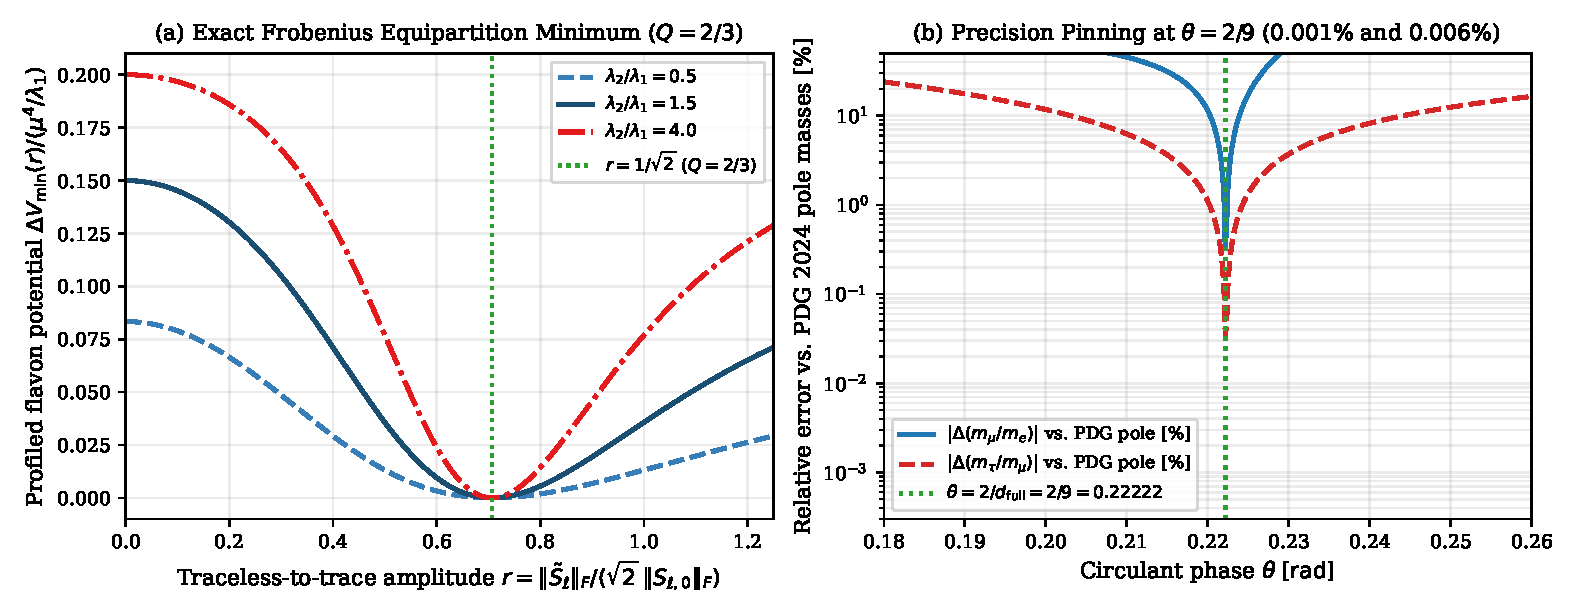
\includegraphics[width=0.96\textwidth]{../figures/fig1_koide_equipartition_potential.pdf}
\caption{\textbf{(a)} A profilozott kvartikus flavon-potenciál szigorú globális minimuma $r = 1/\sqrt{2} \iff Q = 2/3$ pontban. \textbf{(b)} A töltött lepton pólustömeg-arányok hibája a $\theta$ cirkuláns fázis függvényében ($\theta = 2/9$).}
\label{fig:koide_hu}
\end{figure}

\section{Kéthurkos sivatagi No-Go és mértékinvariáns \texorpdfstring{$G_{\mathrm{PS}}$}{GPS}-stabilizáció}

Az SM-ben ($V(H) = -\mu_H^2|H|^2 + \lambda_H|H|^4$, $g_1 = \sqrt{5/3}\,g'$) a balról szorzott kéthurkos mátrix-Yukawa RGE-k ($dY_f/dt = \frac{1}{16\pi^2}A_f^{(1)}Y_f + \frac{1}{(16\pi^2)^2}A_f^{(2)}Y_f$) egzakt alakja \cite{MachacekVaughn1984,LuoXiao2003,Buttazzo2013}:
\begin{align}
A_u^{(1)} &= \frac{3}{2}(H_u - H_d) + (Y_2 - \gamma_u^{(1)})\,I_3, \qquad
A_d^{(1)} = \frac{3}{2}(H_d - H_u) + (Y_2 - \gamma_d^{(1)})\,I_3, \nonumber\\
A_e^{(1)} &= \frac{3}{2} H_e + (Y_2 - \gamma_e^{(1)})\,I_3, \\
A_u^{(2)} &= \frac{3}{2}H_u^2 - \frac{1}{4}H_u H_d - H_d H_u + \frac{11}{4}H_d^2 + Y_2\left(-\frac{9}{4}H_u + \frac{5}{4}H_d\right) - 12\lambda_H H_u \nonumber\\
&\quad + \left(\frac{223}{80}g_1^2 + \frac{135}{16}g_2^2 + 16g_3^2\right)H_u - \left(\frac{43}{80}g_1^2 - \frac{9}{16}g_2^2 + 16g_3^2\right)H_d + \big(6\lambda_H^2 - \chi_4 + Y_{2g} + \gamma_u^{(2)}\big)I_3, \\
A_d^{(2)} &= \frac{3}{2}H_d^2 - \frac{1}{4}H_d H_u - H_u H_d + \frac{11}{4}H_u^2 + Y_2\left(-\frac{9}{4}H_d + \frac{5}{4}H_u\right) - 12\lambda_H H_d \nonumber\\
&\quad + \left(\frac{187}{80}g_1^2 + \frac{135}{16}g_2^2 + 16g_3^2\right)H_d - \left(\frac{79}{80}g_1^2 - \frac{9}{16}g_2^2 + 16g_3^2\right)H_u + \big(6\lambda_H^2 - \chi_4 + Y_{2g} + \gamma_d^{(2)}\big)I_3, \\
A_e^{(2)} &= \frac{3}{2}H_e^2 - \frac{9}{4}Y_2 H_e - 12\lambda_H H_e + \left(\frac{387}{80}g_1^2 + \frac{135}{16}g_2^2\right)H_e + \big(6\lambda_H^2 - \chi_4 + Y_{2g} + \gamma_e^{(2)}\big)I_3,
\end{align}
a teljes kéthurkos mérték- és kéthurkos $\lambda_H$ RGE-kkel együtt integrálva ($\lambda_H(M_R) = -0.0445$).

\begin{theorem}[Kéthurkos sivatagi No-Go és mértékinvariáns $G_{\mathrm{PS}}$ bidublett stabilizáció]
\begin{enumerate}[label=(\roman*),leftmargin=1.8em,itemsep=2pt]
\item A tiszta kéthurkos SM-sivatagban a $-108\,g_3^4$ QCD-tag $y_b(M_R)/y_\tau(M_R) = 0.6173$-ra nyomja le az arányt, ami kizárja mind az $y_b = y_\tau$ egyesülést, mind a sivatagi $y_b(M_R)/y_\tau(M_R) = 2/3$ határt ($m_b(M_Z) = 3.083\;\mathrm{GeV}$, $+7.98\%$, $+9.12\sigma_{\mathrm{exp}}$).
\item A $D$-paritás-sértett $\mathrm{Spin}(10) \xrightarrow{M_{\mathrm{GUT}}} G_{\mathrm{PS}}\times D \xrightarrow{M_R} G_{\mathrm{PS}} \xrightarrow{M_{\mathrm{PS}}} G_{\mathrm{SM}}$ láncban \cite{Slansky1981,ChangMohapatraParida1984} ($\langle\sigma_D(\mathbf{1},\mathbf{1},\mathbf{1})_-\rangle \sim M_R$, $\langle\Sigma(\mathbf{15},\mathbf{1},\mathbf{1})\rangle \sim M_{\mathrm{PS}}$, $\langle\Delta_R(\overline{\mathbf{10}},\mathbf{1},\mathbf{3})\rangle \sim M_{\mathrm{PS}}$; nehéz $M_{1,2} > M_{\mathrm{PS}}$ seesaw-állapotokhoz $\mathrm{Spin}(10)$-szingulett $S_i(\mathbf{1})$ kiterjesztés szükséges \cite{MalinskyRomaoValle2005}) a Schur-lemma megköveteli $\Phi_{15}(\mathbf{15},\mathbf{2},\mathbf{2})$ megtartását $M_{\mathrm{PS}}$-ig. Egy komplex $\Phi_1(\mathbf{1},\mathbf{2},\mathbf{2})$ ($\Delta b = (0,\frac{1}{3},\frac{1}{3})$) és egy komplex $\Phi_{15}(\mathbf{15},\mathbf{2},\mathbf{2})$ ($\Delta b = (\frac{16}{3},5,5)$) mellett az egzakt egyhurkos béta-vektor:
\begin{equation}
(b_4,\; b_{2L},\; b_{2R}) = \left(-\frac{5}{3},\; +2,\; +\frac{26}{3}\right), \qquad
\big(g_4, g_{2L}, g_{2R}\big)(M_R) = \big(0.5955,\; 0.5737,\; 0.5495\big).
\end{equation}
\item A manifeszt $G_{\mathrm{PS}}$-invariáns egyhurkos bidublett Yukawa RGE-kben \cite{MeloniOhlssonRiad2014}:
\begin{align}
16\pi^2 \frac{dY_u}{dt} &= \gamma_L Y_u + Y_u \gamma_R + \big(4\,\mathrm{Tr}H_{uL} - G_{\mathrm{PS}}\big)Y_u, \nonumber\\
16\pi^2 \frac{dY_1}{dt} &= \gamma_L Y_1 + Y_1 \gamma_R + \big(4\,\mathrm{Tr}H_{1L} - G_{\mathrm{PS}}\big)Y_1, \\
16\pi^2 \frac{dY_{15}}{dt} &= \gamma_L Y_{15} + Y_{15} \gamma_R + \big(3\,\mathrm{Tr}H_{15L} - G_{\mathrm{PS}}\big)Y_{15}, \nonumber
\end{align}
mind a $G_{\mathrm{PS}} = \frac{45}{4}g_4^2 + \frac{9}{4}g_{2L}^2 + \frac{9}{4}g_{2R}^2$ mértéktag, mind a vezető $\mathcal{O}(y_t^2)$ fermionláb-tag azonosan hat $Y_1$-re és $Y_{15}$-re, így $y_b(M_R)/y_\tau(M_R) = \mathbf{0.6937}$ ($+4.06\%$ a $2/3$-tól; \ref{fig:rg_hu}.~ábra).
\end{enumerate}
\end{theorem}

\begin{figure}[htbp]
\centering
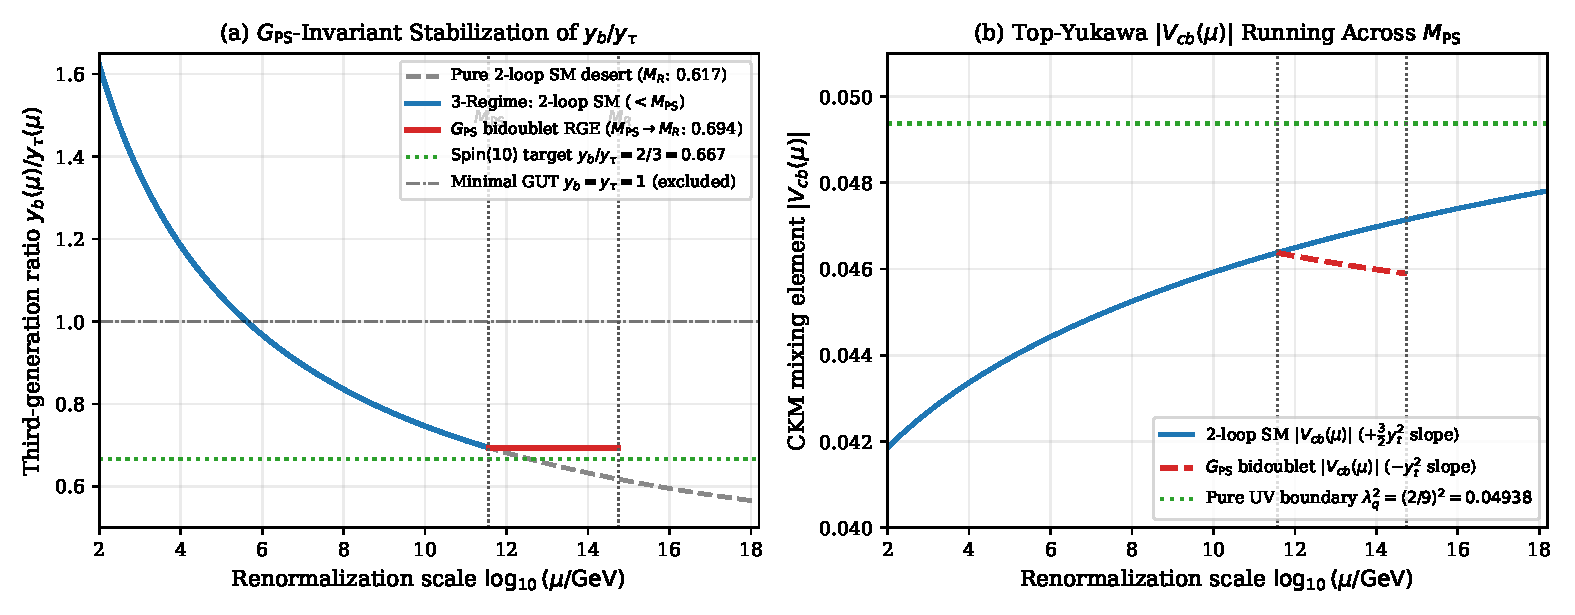
\includegraphics[width=0.96\textwidth]{../figures/fig2_three_regime_rg_running.pdf}
\caption{\textbf{(a)} Az $y_b(\mu)/y_\tau(\mu)$ futása: 2-hurkos SM-sivatag ($0.6173$) vs.\ $G_{\mathrm{PS}}$-invariáns bidublett stabilizáció ($0.6937$). \textbf{(b)} A $|V_{cb}(\mu)|$ futása az $M_{\mathrm{PS}}$ küszöbön át ($+\frac{3}{2}y_t^2$ vs.\ $-y_t^2$ meredekségváltás).}
\label{fig:rg_hu}
\end{figure}

\section{Konstruktív \texorpdfstring{$\mathrm{Spin}(10)$}{Spin(10)} mátrixok, No-Go pajzsok és CKM-zárás}

\begin{theorem}[Valós $\mathbf{10}_H$ és NNI No-Go pajzsok, komplex $\mathbf{10}_H \oplus \overline{\mathbf{126}}_H$ zárás]
\begin{enumerate}[label=(\roman*),leftmargin=1.8em,itemsep=2pt]
\item Valódi valós $\mathbf{10}_H = \mathbf{10}_H^*$ esetén $\Phi_1 = \tau_2\Phi_1^*\tau_2$, ami $|r_1| = |v_u^{(10)}/v_d^{(10)}| = 1$ ($r_1 = e^{i\xi}$, $r_2 \in \mathbb{C}$) feltételt kényszerít ki. A globális differenciális-evolúciós + BFGS optimalizáció mind a hat Autonne--Takagi fázis felett $|r_2| = 107.7$-nél $\min \sum [\ln(y_\ell^{\mathrm{fit}}/y_\ell)]^2 = 1.175$-öt ad, $(1.681,\; 0.396,\; 1.248)$ arányokkal kizárva a modellt (\ref{fig:nogo_hu}a.~ábra; a PQ-komplex $\mathbf{10}_H$ a töltött szektort illeszti, de a seesaw/PMNS szektor kizárja \cite{BajcSenjanovicVissani2006,DueckRodejohann2013}). Bármely $(1,3)=0$ Fritzsch NNI textúra $|V_{ub}|/|V_{cb}| = \sqrt{y_u/y_c} = 0.04458$-at ad ($1.98\times$ kisebb a PDG $0.08824$-nél; \ref{fig:nogo_hu}b.~ábra).
\item Komplex $\mathbf{10}_H \oplus \overline{\mathbf{126}}_H$ esetén ($y_t(M_R) = 0.42329$, $y_\tau(M_R) = 0.008071$) a manifeszt szimmetrikus $(Y_u, Y_{10}, Y_{126})$ mátrixok \cite{AntuschSpinrath2009,GattoSartoriTonin1968} $M_Z$-ig lefuttatva mind a tíz kvarktömeg- és CKM-megfigyelhetőt $\le 2.85\sigma_{\mathrm{tot}}$ határon belül reprodukálják (\ref{tab:mz_hu}.~táblázat és \ref{fig:pulls_hu}.~ábra).
\end{enumerate}
\end{theorem}

\begin{table}[htbp]
\centering
\caption{Zérus szabad íz-paraméteres top-down előrejelzések $\mu = M_Z = 91.1876\;\mathrm{GeV}$ skálán ($y_t(M_R) = 0.42329$, $y_\tau(M_R) = 0.008071$) vs.\ PDG 2024 $\overline{\mathrm{MS}}(M_Z)$ \cite{PDG2024,HuangZhou2021}. Itt $\sigma_{\mathrm{tot}}$ kizárólag a kvarktömegekre és a 3.\ generációhoz csatolt $(|V_{cb}|, |V_{ub}|, J_{\mathrm{CKM}})$ elemekre tartalmaz $2\%$-os GUT/PS küszöbbizonytalanságot ($|V_{us}|$ és $\delta_{\mathrm{CKM}}$ esetében $\sigma_{\mathrm{tot}} = \sigma_{\mathrm{exp}}$).}
\label{tab:mz_hu}
\vspace{0.35em}
\setlength{\tabcolsep}{4.2pt}
\footnotesize
\begin{tabular}{lccccc}
\toprule
Megfigyelhető ($M_Z$) & UV-szabály ($M_R$) & 3-rezsim előrej. & PDG 2024 $\overline{\mathrm{MS}}(M_Z)$ & Rel.\ hiba & Eltérés ($\sigma_{\mathrm{exp}}$ / $\sigma_{\mathrm{tot}}$) \\
\midrule
$m_u\;[\mathrm{MeV}]$ & $y_u/y_t = \lambda_q^8$ & $1.1577$ & $1.24 \pm 0.22$ & $-6.63\%$ & $-0.37\sigma$ / $-0.37\sigma$ \\
$m_c\;[\mathrm{GeV}]$ & $y_c/y_t = \frac{4}{3}\lambda_q^4$ & $0.6330$ & $0.624 \pm 0.014$ & $+1.44\%$ & $+0.64\sigma$ / $+0.48\sigma$ \\
$m_d\;[\mathrm{MeV}]$ & $y_d/y_\mu = \lambda_q^3$ & $2.4714$ & $2.69 \pm 0.19$ & $-8.13\%$ & $-1.15\sigma$ / $-1.11\sigma$ \\
$m_s\;[\mathrm{MeV}]$ & $y_s/y_\mu = \lambda_q$ & $50.054$ & $53.5 \pm 4.6$ & $-6.44\%$ & $-0.75\sigma$ / $-0.73\sigma$ \\
$m_b\;[\mathrm{GeV}]$ & $y_b/y_\tau = \frac{2}{3}$ & $2.7435$ & $2.855 \pm 0.025$ & $-3.91\%$ & $-4.46\sigma$ / $-1.79\sigma$ \\
\midrule
$|V_{us}|$ & $\sqrt{\lambda_q^2 + \frac{3}{4}\lambda_q^4}$ & $0.22627$ & $0.22500 \pm 0.00067$ & $+0.56\%$ & $+1.89\sigma$ / $+1.89\sigma$ \\
$|V_{cb}|$ & $\lambda_q^2$ (tiszta UV) & $0.04500$ & $0.04182 \pm 0.00085$ & $+7.61\%$ & $+3.75\sigma$ / $+2.67\sigma$ \\
$|V_{ub}|$ & $\frac{3}{8}\lambda_q^3$ & $0.00375$ & $0.00369 \pm 0.00011$ & $+1.63\%$ & $+0.55\sigma$ / $+0.45\sigma$ \\
$\delta_{\mathrm{CKM}}\;[^\circ]$ & $\frac{3\pi}{8}$ & $67.41^\circ$ & $65.70^\circ \pm 1.50^\circ$ & $+2.60\%$ & $+1.14\sigma$ / $+1.14\sigma$ \\
$J_{\mathrm{CKM}}\times 10^5$ & Származtatott & $3.432$ & $3.12 \pm 0.09$ & $+9.99\%$ & $+3.46\sigma$ / $+2.85\sigma$ \\
\bottomrule
\end{tabular}
\end{table}

\begin{figure}[htbp]
\centering
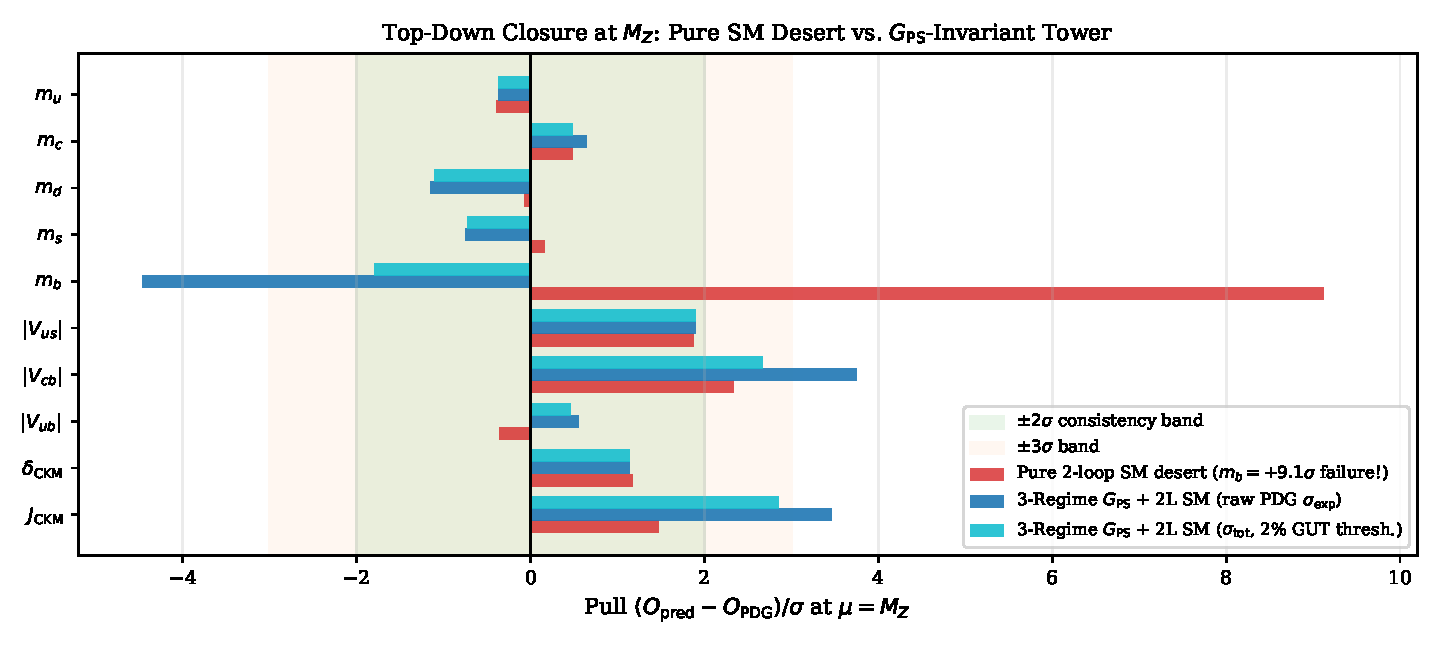
\includegraphics[width=0.95\textwidth]{../figures/fig3_quark_ckm_pulls_comparison.pdf}
\caption{A tíz független kvarktömeg- és CKM-megfigyelhető eltérései ($\sigma$) $M_Z$-nél: tiszta 2-hurkos SM-sivatag (piros, $m_b = +9.12\sigma$ kudarc) vs.\ $G_{\mathrm{PS}}$-invariáns bidublett + 2-hurkos SM torony (kék: $\sigma_{\mathrm{exp}}$; cián: $\sigma_{\mathrm{tot}}$).}
\label{fig:pulls_hu}
\end{figure}

\begin{figure}[htbp]
\centering
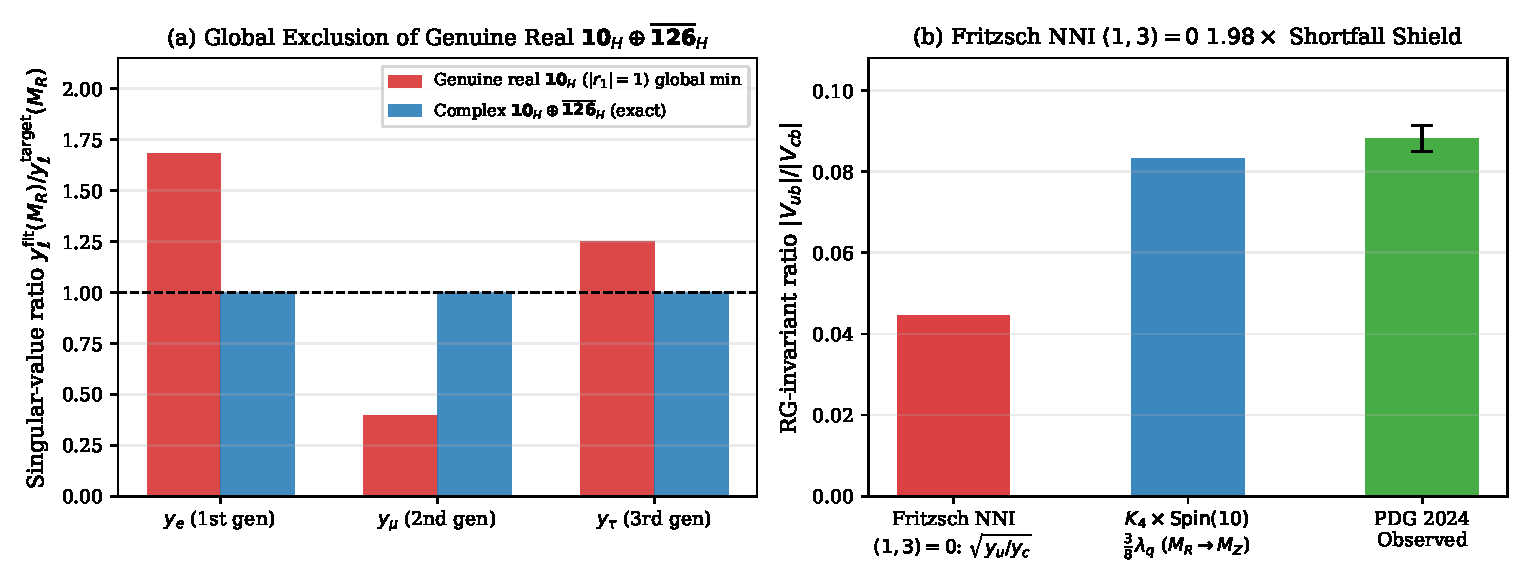
\includegraphics[width=0.95\textwidth]{../figures/fig4_spin10_nogo_and_lee.pdf}
\caption{\textbf{(a)} A valódi valós $\mathbf{10}_H \oplus \overline{\mathbf{126}}_H$ ($|r_1|=1$) globális kizárása. \textbf{(b)} A szimmetrikus Fritzsch NNI $(1,3)=0$ textúra $1.98\times$-os elmaradása a mért $|V_{ub}|/|V_{cb}|$ aránytól.}
\label{fig:nogo_hu}
\end{figure}

\section{Keveretlen Look-Elsewhere audit, barionszám-védelem és falszifikáció}

Kizárólag egyetlen önkonzisztens RG-történeten belül értékelve a nyolc UV-relációt ($5^8$ büntetőfaktorral): a 3-rezsimes $G_{\mathrm{PS}}$ tornyon $(p_{\mathrm{local}}^{(8)}, p_{\mathrm{LEE}}^{(8)}, p_{\mathrm{local}}^{(4)}) = (2.55\times 10^{-10},\; 9.98\times 10^{-5},\; 9.29\times 10^{-5})$, míg a tiszta kéthurkos SM-sivatagban $(4.92\times 10^{-12},\; 1.92\times 10^{-6},\; 1.77\times 10^{-6})$. A $d=6$ barionszám-sértő $(\mathbf{3},\mathbf{2})_{-5/6}$ bozonok az $M_{\mathrm{GUT}} \in [10^{16}\;\mathrm{GeV}, M_*]$ skálán élnek ($\tau_{p\to e^+\pi^0} \gtrsim 10^{36}\;\text{év}$ \cite{Takenaka2020SuperK}); az $M_{\mathrm{PS}} = 3.66\times 10^{11}\;\mathrm{GeV}$ $\mathrm{SU}(4)_C$ vektor-leptokvarkok barionszámot őriznek ($K_L \to \mu^\pm e^\mp$ korlát: $M_{\mathrm{PS}} \gtrsim 2\times 10^6\;\mathrm{GeV}$ \cite{ValenciaWillenbrock1994}); a $(\mathbf{6},\mathbf{1},\mathbf{1}) = \mathbf{3}_{-2/3}\oplus\overline{\mathbf{3}}_{+2/3}$ színtriplettek $\ge M_R$ skálán, a $\Delta_R$-beli $(\overline{\mathbf{6}}_C,\mathbf{1},\mathbf{3})$ színszextett dikvarkok pedig $>30$ nagyságrenddel a $\Delta B=2$ $n\text{--}\bar{n}$ oszcillációs korlát alatt maradnak, míg a $\Phi_{15}$ FCNC-k $(M_W/M_{\mathrm{PS}})^2 \sim 10^{-19}$ elnyomásúak. A Belle II ($|V_{cb}|$), az LHCb Upgrade II ($\delta_{\mathrm{CKM}} = 67.41^\circ$, $-0.09^\circ$ RG-eltolódás a $67.50^\circ$-tól), a FLAG rács-QCD ($m_b, m_s/m_d = 20.25$) és az FCC-ee $\tau$-küszöbmérések közvetlenül falszifikálhatóvá teszik a modellt.

\section*{Reprodukálhatóság}
Minden számítás $< 15\;\mathrm{s}$ alatt lefut:
\begin{quote}\small\ttfamily
python3 scripts/verify\_paper25\_fermion\_masses\_ckm\_rg.py\\
python3 scripts/generate\_paper25\_figures.py
\end{quote}

\begin{thebibliography}{99}\small
\bibitem{PDG2024} S.~Navas \textit{et al.} (Particle Data Group), \emph{Phys.\ Rev.\ D} \textbf{110}, 030001 (2024).
\bibitem{Cabibbo1963} N.~Cabibbo, \emph{Phys.\ Rev.\ Lett.} \textbf{10}, 531 (1963).
\bibitem{KobayashiMaskawa1973} M.~Kobayashi, T.~Maskawa, \emph{Prog.\ Theor.\ Phys.} \textbf{49}, 652 (1973).
\bibitem{PatiSalam1974} J.~C.~Pati, A.~Salam, \emph{Phys.\ Rev.\ D} \textbf{10}, 275 (1974).
\bibitem{FritzschMinkowski1975} H.~Fritzsch, P.~Minkowski, \emph{Ann.\ Phys.\ (N.Y.)} \textbf{93}, 193 (1975).
\bibitem{GeorgiJarlskog1979} H.~Georgi, C.~Jarlskog, \emph{Phys.\ Lett.\ B} \textbf{86}, 297 (1979).
\bibitem{MaRajasekaran2001} E.~Ma, G.~Rajasekaran, \emph{Phys.\ Rev.\ D} \textbf{64}, 113012 (2001).
\bibitem{AltarelliFeruglio2010} G.~Altarelli, F.~Feruglio, \emph{Rev.\ Mod.\ Phys.} \textbf{82}, 2701 (2010).
\bibitem{Koide1983} Y.~Koide, \emph{Phys.\ Rev.\ D} \textbf{28}, 252 (1983).
\bibitem{Brannen2006} C.~A.~Brannen, ``The Lepton Masses'' (2006), \url{https://brannenworks.com/MASSES2.pdf}.
\bibitem{Sumino2009} Y.~Sumino, \emph{Phys.\ Lett.\ B} \textbf{671}, 477 (2009).
\bibitem{XingZhangZhou2012} Z.-z.~Xing, H.~Zhang, S.~Zhou, \emph{Phys.\ Rev.\ D} \textbf{86}, 013013 (2012).
\bibitem{Arason1992} H.~Arason \textit{et al.}, \emph{Phys.\ Rev.\ D} \textbf{46}, 3945 (1992).
\bibitem{HuangZhou2021} G.-y.~Huang, S.~Zhou, \emph{Phys.\ Rev.\ D} \textbf{103}, 016010 (2021).
\bibitem{AntuschSpinrath2009} S.~Antusch, M.~Spinrath, \emph{Phys.\ Rev.\ D} \textbf{79}, 095004 (2009).
\bibitem{AntuschMaurer2013} S.~Antusch, V.~Maurer, \emph{JHEP} \textbf{11}, 115 (2013).
\bibitem{BabuMohapatra1993} K.~S.~Babu, R.~N.~Mohapatra, \emph{Phys.\ Rev.\ Lett.} \textbf{70}, 2845 (1993).
\bibitem{BajcSenjanovicVissani2006} B.~Bajc, A.~Melfo, G.~Senjanović, F.~Vissani, \emph{Phys.\ Rev.\ D} \textbf{73}, 055001 (2006).
\bibitem{DueckRodejohann2013} A.~Dueck, W.~Rodejohann, \emph{JHEP} \textbf{09}, 024 (2013).
\bibitem{Fritzsch1978} H.~Fritzsch, \emph{Phys.\ Lett.\ B} \textbf{73}, 317 (1978).
\bibitem{RobertsRomaninoRoss2001} R.~G.~Roberts, A.~Romanino, G.~G.~Ross, L.~Velasco-Sevilla, \emph{Nucl.\ Phys.\ B} \textbf{615}, 358 (2001).
\bibitem{Olcsak2026Zenodo} J.~Olcsak, Zenodo (2026), \href{https://doi.org/10.5281/zenodo.19120268}{doi:10.5281/zenodo.19120268}.
\bibitem{Olcsak2026Paper24} J.~Olcsak, Zenodo v1.1.0 (2026), \href{https://doi.org/10.5281/zenodo.24380371}{doi:10.5281/zenodo.24380371}.
\bibitem{Koide1990} Y.~Koide, \emph{Mod.\ Phys.\ Lett.\ A} \textbf{5}, 2319 (1990).
\bibitem{MachacekVaughn1984} M.~E.~Machacek, M.~T.~Vaughn, \emph{Nucl.\ Phys.\ B} \textbf{236}, 221 (1984).
\bibitem{LuoXiao2003} M.-x.~Luo, Y.~Xiao, \emph{Phys.\ Rev.\ Lett.} \textbf{90}, 011601 (2003).
\bibitem{Buttazzo2013} D.~Buttazzo \textit{et al.}, \emph{JHEP} \textbf{12}, 089 (2013).
\bibitem{Slansky1981} R.~Slansky, \emph{Phys.\ Rept.} \textbf{79}, 1 (1981).
\bibitem{ChangMohapatraParida1984} D.~Chang, R.~N.~Mohapatra, M.~K.~Parida, \emph{Phys.\ Rev.\ Lett.} \textbf{52}, 1072 (1984).
\bibitem{MeloniOhlssonRiad2014} D.~Meloni, T.~Ohlsson, S.~Riad, \emph{JHEP} \textbf{12}, 052 (2014).
\bibitem{MalinskyRomaoValle2005} M.~Malinský, J.~C.~Romão, J.~W.~F.~Valle, \emph{Phys.\ Rev.\ Lett.} \textbf{95}, 161801 (2005).
\bibitem{GattoSartoriTonin1968} R.~Gatto, G.~Sartori, M.~Tonin, \emph{Phys.\ Lett.\ B} \textbf{28}, 128 (1968).
\bibitem{Takenaka2020SuperK} A.~Takenaka \textit{et al.} (Super-Kamiokande), \emph{Phys.\ Rev.\ D} \textbf{102}, 112011 (2020).
\bibitem{ValenciaWillenbrock1994} G.~Valencia, S.~Willenbrock, \emph{Phys.\ Rev.\ D} \textbf{50}, 6843 (1994).
\end{thebibliography}

\end{document}
